\documentclass{article}
\usepackage[utf8]{inputenc}
\usepackage{authblk}
\usepackage{graphicx}
\usepackage{amsmath, amsfonts, amssymb}
\usepackage{tikz}
\usepackage{hyperref}
\usetikzlibrary{positioning}
\usepackage[table]{xcolor}
\usepackage{listings}



\title{Draft Report Modelleren-B}
\author{Bart Stolk \and Dyami Silvério \and Wessel van Sommeren \and Severijn Wiechers}
\date{03 June 2021}

\begin{document}

\maketitle

%maak een foto foor op de titlepagina

\newpage
\section*{list of variables}
\addcontentsline{toc}{section}{List of variables}
% nog aanvullen


\newpage
\section*{Summary}
\addcontentsline{toc}{section}{Summary}
In this project we explored the world of parcel delivery. Based on a dataset provided we explored various option to optimize the cost of delivering a parcel, this cost optimization was done by building or not building hubs near certain cities. The first algorithm applied was an intuitive algorithm it does not guarantee the optimal solution, but it does give a reasonable solution. The other algorithm applied was an ILP which is takes a lot longer to run but does give the best possible solution.

%mag wat langer // moet opzichzelf het gehele verslag omvatten // alle belangrijke info en conlcusie




\newpage
\tableofcontents



\newpage
\section{Introduction}


% Reducing costs is a valuable tool for any package delivery cooperation to stay relevant and make profits. This report will try to show how it is possible to create an algorithm that gives an optimum case of hubs such that the total cost is minimized % we moeten de hoofdvraag nog even correct opstellen.

Reducing costs is a valuable tool for any package delivery cooperation to stay relevant and make profits. Hereby, algorithms are a useful and necessary tool to optimize a given data set. In this case the goal of the report is to find an algorithm to minimize the cost of a package delivery company. Hereby a data set is used where the different transfer, collection and distribution costs are given per city. The objective of the algorithm is to find the cities where hubs should be build such that the total cost of sending and receiving packages can be brought down to a minimum. An important restraint in this matter is that packages can only move between hubs and cities and in particular not directly between cities themselves. %B: What about flow? // vertellen wat er in de data set staat

Since this type of optimization problem is a common practice for companies, there already exists an ILP solver which can give the exact hubs for which have the lowest total cost, However, it has shown that these solvers can take up and lot of time and processing power. Therefore it is preferable to get an idea for which routes and hubs will give the best, or at least a proper solution to the problem. This will be done by creating different intuitive algorithms which will, if done correctly, give similar results using different methods.

In the first chapter the intuitive algorithms will be explained along with the function which is used to calculate the total costs of choosing a specific combination of hubs. Thereafter, the chapter will set forth the input and result of the ILP Solver. The section in chapter 4 will focus on a reflection between the result of the intuitive algorithm and the solution of the ILP solver. In the following chapter multiple expansions of the problem and intuitive algorithm will be given such that a better result is obtained. Finally, the last chapter will contain a conclusion of the report.






\newpage
\section{Intuitive Algorithm}
\label{Inuitive algorithms}
As mentioned in the introduction, it can be useful to use an intuitive algorithm instead of a direct solver for the problem. With a self made script it is possible to get a feel for the cities in which building a hub can have a major impact on reducing the cost of the project. 
Before a code can be written that tries to optimize the building of hubs in cities, it is necessary to have a solid view of the costs that a specific combination of hubs will bring forth. Therefore a cost-function is written that will give a total cost as output with a combination of hubs as input. 



    \subsection{Calculating the cost for multiple hubs}
        To calculate the cost of using specific hubs we first choose a way to determine connections from hubs to cities. The most intuitive way to determine those connections was to link each city with the hub that was cheapest to collect and distribute to. Intuitively this made sense as it probably the closest. If we take for example the Netherlands this would mean that a package sent from Groningen would be picked up by a hub close to Groningen and not by a hub in for example Maastricht. So the first step in the cost function algorithm was to go trough the list of cities and determine which hub from the list of input hubs was cheapest to collect from for each city. When this connection is determined the sum of the list multiplied by the collection factor and is added to the cost and the the amount of packages are added to the packages of the hub city. %B: Very long, difficult to follow sentence. Split up in 2 maybe?
        
        The connection between the city and collection hub was stored in memory as it would be used later to determine transfers and delivery. As soon as this first step is complete we end up with a Data frame with as columns the hub cities and rows the packages that need to go to each city. The next step is to go row by row and look up what connection that city had with which hub and transfer all the packages of that row to the correct hub again multiplying the amount times the correct cost associated with transferring from hub to hub. Then the total of that row at the correct hub will be delivered to the city and thus multiplying the total number of packages by the cost to deliver from that hub to the city and the delivery factor. Once that is done for all rows, all packages will be delivered. Now we only need to add the cost of building the hubs and we have the total cost of using specific hubs. %iets compacter wellicht
        
        
    \subsection{The different algorithms used}
    
    After obtaining a function which calculates the cost of assigning hubs to cities, an intuitive algorithm can be made which tries to give an approximation of the combination of hubs that will result in the lowest possible amount of money that the company will have to spend when moving packages. 
    Since the intuitive algorithms are inherently less accurate than a standardized solver, the different aspects of moving packages are split up and solved using different types of algorithms. Hereby, the goal is to minimize the error that the functions have by eventually combining multiple intuitive algorithms such that a minimum cost can be achieved. The total process is divided into the collection from the cities to the hubs, followed by the transfer between hubs themselves, and as last the distribution of packages from the hubs to the desired cities. 
    % we moeten misschien nog even de namen van 2.3 2.5 enzo aanpassen aangezien het originele idee van het opsplitsen van collection, transer en distribution  niet meer van toepassing is
    \subsection{Collection of packages}  
    \label{Collection of packages}
    In this process the cost function will only give an output of the cost that is formed by combining the cost for collecting packages. To optimize the costs a python script is made such that, when a city is given to be a hub, the code calculates the cost for this specific hub and the cost if the city next in line would be a hub as well. If the total cost drops by adding city as a hub, this city will be added to list of cities that are hubs. If the cost rises, the city will be discarded from the process. If this process is repeated with each time a different starting node, a list will appear of possible combination of hubs and their costs. To illustrate this process the outputs will be stated below if it were to start with city number 3 as a hub.

    \begin{table}[h!]
        \begin{center}
            \begin{tabular}{||c |c||} 
                \hline
                Cost of the combination(€ x 10^3) & combination on cities as hubs \\ [0.5ex] 
                \hline\hline
                169.3 & [3,1]  \\ 
                \hline
                169.8 & [3,2]  \\
                \hline
                169.8 & [3,4]  \\
                \hline
                127.2 & [3,5]  \\ 
                \hline
                132.0 & [3,5,6]  \\
                \hline
                127.4 & [3,5,7]  \\
                \hline
                128.5 & [3,5,8]  \\
                \hline
                124.8 & [3,5,9]  \\
                \hline
                118.7 & [3,5,9,10]  \\
                [1ex] 
                \hline
              \end{tabular}
          \end{center}
        \caption{Exampled of the algorithm which adds cities one by one as hubs based on the cost}
        \label{Collection Algorithm}
    \end{table}

    Using this method, the algorithm can give the most frequently used cities as hubs. To illustrate the difference in accuracy between the different models the table below will give the amount of times cities are used as hubs in each different part.% Herlezen
    
        \subsubsection{Result of the large data set}
    
            Using the large data set given with 14 different cities, the results are stated below. 
    
            \begin{table}[h!]
                \begin{center}
                \begin{tabular}{|p{3cm}|p{3cm}|p{3cm}|}
                    \hline
                    \multicolumn{3}{|c|}{Amount of times cities are used as hubs} \\
                    \hline
                    City used as hub & Using only collection cost & Using total cost\\
                    \hline
                    1 &  8 & 5 \\
                    \hline
                    2 & 4   & 11 \\
                    \hline
                    3& 7 & 9\\
                    \hline
                    4  & 1 & 1 \\
                    \hline
                    5 & 8 & 9\\
                    \hline
                    6 & 1 & 8   \\
                    \hline
                    7 & 2& 3 \\
                    \hline
                    8 & 2 & 2 \\
                    \hline
                    9 &  7& 10 \\
                    \hline
                    10 & 11 & 11 \\
                    \hline
                    11 & 1& 2 \\
                    \hline
                    12 & 1 & 1 \\
                    \hline
                    13 & 2& 2 \\
                    \hline
                    14 & 14& 14 \\
                    \hline
                \end{tabular}
                \end{center}
                \caption{Table of the amount of times each city is used as a hub in every combination using the large data set}
                \label{amount of times hubs are used in collection} 
            \end{table}
    
            Using this table a conclusion can be drawn which hubs could be used in the optimum configuration. However, a big part of cost reduction is the combination of specific hubs. Consider city number 6 for example, here it shows that making this city a hub is not a valuable if the algorithm only takes the collection cost in account, but rises significantly if all cost are calculated. 
            
            When the algorithm is used for different input combinations based on ~\ref{amount of times hubs are used in collection} the outputs and results show different possible answers with supposedly relative low cost. Hereby the algorithm will add a city as hub if this results in a lower cost by the principle given in the beginning of the section. 
    
            \begin{table}[h!]
                \begin{center}
                    \begin{tabular}{ |p{3cm}|p{3cm}|p{4cm}|}
                        \hline
                        \multicolumn{3}{|c|}{Cost and combination of hubs with certain input} \\
                        \hline
                        Input into the algorithm & Output -  collection Cost (€ x 10^3) & Output - total Cost (€ x 10^3)\\
                        \hline
                        [14] &  92.6 | [14, 1, 3] & 166.4 | [14, 1, 2, 3, 5, 7]  \\
                        \hline
                        [10] & 90.0 | [10, 2, 14]   & 153.0 | [10, 2, 14, 8] \\
                        \hline
                        [6, 10]& 93.9 | [6, 10, 14] & 150.4 |  [6, 10, 14]\\
                        \hline
                        [6, 14] &  82.9 | [6, 14]  &  144.5 | [6, 14, 8] \\
                        \hline
                        [9, 14] &  100.7| [9, 14, 1, 3] & 160.4 |  [9, 14, 2, 3, 7] \\
                        \hline
                        [2, 14] & 87.6 | [2, 14, 6] & 156.9 |  [2, 14, 3, 6]\\
                        \hline
                        [2, 10, 14] & 90.0 | [2, 10, 14] & 153.0 | [2, 10, 14, 8]  \\
                        \hline
                    \end{tabular}
                \end{center}
            \caption{Table of the amount of times each city is used as a hub in every combination}
            \label{amount of times hubs are used in collection} 
            \end{table}
    
            The combination of cities 6, 8 and 14 will probably have one of the lower possible costs for this problem for as well the collection cost as the total cost. Using this combination it shows that the cost can be reduced to around 145 thousand euros. 

        \subsubsection{Result of the small data set}
            For the small data set the same method is used as for the large file. First the amount of times a cities is added as a hub is counted. Thereafter, the result we be run again by the algorithm with the most common cities as hubs to create an optimal solution.
            
             \begin{table}[h!]
                \begin{center}
                \begin{tabular}{|p{3cm}|p{3cm}|p{3cm}|}
                    \hline
                    \multicolumn{3}{|c|}{Amount of times cities are used as hubs} \\
                    \hline
                    City used as hub & Using only collection cost & Using total cost\\
                    \hline
                    1 &  8 & 5 \\
                    \hline
                    2 & 4   & 11 \\
                    \hline
                    3& 7 & 9\\
                    \hline
                    4  & 1 & 1 \\
                    \hline
                    5 & 8 & 9\\
                    \hline
                    6 & 1 & 8   \\
                    \hline
                    7 & 2& 3 \\
                    \hline
                    8 & 2 & 2 \\
                    \hline
                    9 &  7& 10 \\
                    \hline
                    10 & 11 & 11 \\
                    \hline
                \end{tabular}
                \end{center}
                \caption{Table of the amount of times each city is used as a hub in every combination with the small data set}
                \label{amount of times hubs are used in collection} 
            \end{table}
            


    \subsection{Transfer between hubs} \label{sssec:num1}
        Transport to the same node is free if the node is a hub. To optimize the total cost an algorithm is made that will look at the node with the most flow of parcels to itself and makes a hub of this node. After calculating the cost, the next hub with the most flow of parcels to itself will be become a hub. If the solution becomes cheaper by adding a hub, the node is added to a list of hubs. If the total cost increases, nothing happens and the next node (most parcels to itself) becomes a hub. If there are two nodes with the same amount of parcels to itself the algorithm will choose the node with the most incoming parcels. Each node will be connected to the hub with the least cost to transport it there, for example if it cost 11 dollars to transport from node 11 to hub 14 and 27 dollars to transport it to hub 2, node 11 will be connected with hub 14. This process is repeated until the algorithm goes through all nodes. To illustrate we will use the Large and small data assignment.
\subsubsection{Result of the large data set}
        \begin{table}[h!]
            \begin{tabular}{|p{3cm}|p{3cm}|p{3cm}|}
                \hline
                nodes that are hubs & flow of parcels to itself (last node) & Total cost (€ x 10^3)\\
                \hline
                [14] &  181 & 182.7 \\
                \hline
                [14,2]   & 39 & 163.5 \\
                \hline
                [14,2,15] & 26 & 169.3 \\
                \hline
                [14,2,15,6]  & 18 & 156.5 \\
                \hline
                [14,2,15,6,13] & 18 & 161.5\\
                \hline
                [14,2,15,6,13,4] & 11 & 167.0   \\
                \hline
                [14,2,15,6,13,4,3] & 9 & 177.1   \\
                \hline
                [14,2,15,6,13,4,3,9] & 9 & 187.7    \\
                \hline
            \end{tabular}
        \caption{Table of nodes that were used as hubs and the associated costs}
        \end{table}


The cheapest situation here is where there are 4 hubs in nodes 2,6,14 and 15. We connect each node with the hub where the cost to transport a parcel is the lowest, the total cost in this situation would be €156.5 thousand. One can easily see that it is very profitable to make a hub out of node 14, as it is the node with the most incoming parcels (610). In the following subsections we will be looking at the results of the other algorithms and combine those to see if there are similarities.
\subsubsection{Result of the small data set}
(The results of the small data set are still being worked on, though this will be done identically to the large data set.)

\subsection{Distribution of packages}
\label{Distribution}
The idea of minimising the cost of distributing packages is similar to that of collecting packages. However, a somewhat different algorithm was used to do so. First, the algorithm iterates over the cities. For each city, it calculates the cost of having that city as a hub using the cost function. After going through all the cities, the algorithm picks the city which generates the lowest cost and `permanently' adds this city to the list of hubs. Then the algorithm repeats the first few steps, iterating over the cities (excluding the one that has been added as hub already) and calculate which of those costs the least to add. This results in a list of 15 results for the large data set and 10 for the small data set, with each with of the results having one more hub than the one before it. 

It is the expectation that the first few results will result in lower costs. But, once you start adding `too many' hubs, the costs will start rising again. Though this is not assumed to be necessarily true, so the algorithm keeps running until all of the cities have been added as hubs. 

\subsubsection{Result of the large data set}
First, the algorithm was run to minimise distribution costs for the large data set. In table \ref{DistAlg}. To prevent repeating the entire list of hubs, the `Chosen hub' column will only include the hub that was added in that iteration of the algorithm. The costs have also been formulated in thousands rounded to 1 decimal for readability.

\begin{table}[h]
\centering
\begin{tabular}{||c|c|c||}
\hline
    Chosen hub & Total distribution costs (€ x 10^3)& Total costs (€ x 10^3)  \\
\hline
\hline
    10 & 64.2 & 169.2 \\
    \hline
    2 & 48.4 & 166.2 \\
    \hline
    14 & 35.6 & 153.3 \\
    \hline
    8 & 27.7 & 153.0 \\
    \hline
    9 & 22.0 & 159.6 \\
    \hline
    4 & 17.2 & 168.3 \\
    \hline
    6 & 13.9 & 173.3 \\
    \hline
    3 & 11.0 & 183.2 \\
    \hline
    1 & 8.2 & 192.2 \\
    \hline
    13 & 6.3 & 200.3 \\
    \hline
    12 & 4.8 & 208.0 \\
    \hline
    5 & 2.0 & 217.1 \\
    \hline
    11 & 0.9 & 230.2 \\
    \hline
    15 & 0 & 241.0 \\
    \hline
\end{tabular}
\caption{\centering Order in which the cities got added as hubs by the algorithm based on distribution costs}
\label{DistAlg}
\end{table}

As can be seen, the distribution costs decrease with each added hub until they reach 0. This is a result of distribution costs from hubs to themselves costs 0. So more of the actual costs are made up of transfer costs as more hubs get added. However, the total costs, displayed in the last column, have quite different results. At first, the costs decrease. But, after adding hub 9 the total costs increase from there onward. So, based on these results, a solution would be to pick hubs 2, 8, 10 and 14 with a total cost of 152974.

The algorithm was also used based on total costs to compare how much the results differed from basing it on solely distribution costs, the results of which can be found in table \ref{DistAlg2}. With this, the hubs 6, 10 and 14 form an optimal solution. Interestingly, the order in which certain hubs appear in this version is somewhat similar to when it was based on just distribution costs. For example, the first 5 hubs to be added in both cases are the same, namely 2, 6, 8, 10 and 14. Even though their order is different. From this we might conclude that these cities are attractive candidates to be hubs in general.

\begin{table}[h]
\centering
\begin{tabular}{||c|c||}
\hline
    Chosen hub & Total costs (€ x 10^3) \\
\hline
\hline
    10 & 169.3 \\
    \hline
    14 & 156.3 \\
    \hline
    6 & 150.4 \\
    \hline
    8 & 153.2 \\
    \hline
    2 & 156.9 \\
    \hline
    5 & 161.6 \\
    \hline
    13 & 169.0 \\
    \hline
    12 & 178.7 \\
    \hline
    4 & 185.3 \\
    \hline
    1 & 194.3 \\
    \hline
    3 & 204.3 \\
    \hline
    7 & 216.4 \\
    \hline
    9 & 229.2 \\
    \hline
    11 & 242.3 \\
    \hline
    15 & 247.2 \\
    \hline
\end{tabular}

\caption{\centering Order in which the cities got added as hubs by the algorithm based on total costs}
\label{DistAlg2}
\end{table}
\subsubsection{Result of the small data set}
(The results of the small data set are still being worked on, though this will be done identically to the large data set.)




\newpage

    
    \subsection{Result of the combined algorithms}
    \subsubsection{Result of the large data set}
By combining and analysing the results of the different algorithms, a hub will be opened at nodes 14 and 6 as these nodes were also hubs in the cheapest situation of all different algorithms that were used. By opening a hub at node 14 the cost for collecting , transferring and distributing can be reduced, as it is the node with the most amount of incoming parcels. The total cost in this situation where we only have two hubs is €144.870. The intuitive algorithm will then go through the nodes one by one and check which combination (with node 14 and 6) is the cheapest, this node will then be added to the list of hubs. This process is repeated until the algorithm goes through all nodes. 

\begin{table}[h]
\begin{tabular}{||c |c||}
\hline
Nodes that are hubs & Total cost (€ x 10^3)\\
\hline
[6,14] &  144.8 \\
\hline
[6,8,14]   & 144.5\\
\hline
[2,6,8,14] & 148.1 \\
\hline
[2,5,6,8,14]  & 152.5  \\
\hline
[2,5,6,8,12,14] & 160.3 \\
\hline
\end{tabular}
\caption{Table of nodes that were used as hubs in the initiative algorithm}
\end{table}

The most advantageous situation that was found with the intuitive algorithm is 
where we make 3 hubs out of nodes 6,8 and 14. By doing this the total cost is reduced to €144.532 which is €338 cheaper than the previous one. 

\begin{figure}[h]
\centering
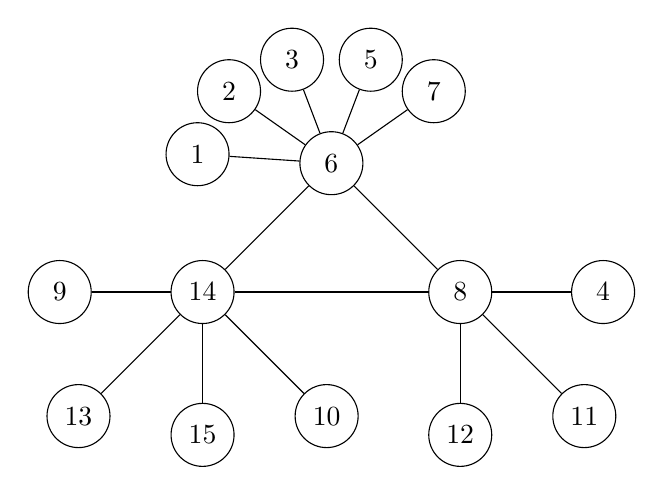
\begin{tikzpicture}[main/.style = {draw, circle,minimum size=0.8cm}]
\node[main] (6) {6};
\node[main] (8) [below right=1.5cm of 6] {8};
\node[main] (14) [below left=1.5cm of 6] {14};

\node[main] (1) [above=of 6,xshift=-1.7cm,yshift=-1.7cm] {1};
\node[main] (2) [above=of 6,xshift=-1.3cm,yshift=-0.9cm] {2};
\node[main] (3) [above=of 6,xshift=-0.5cm,yshift=-0.5cm] {3};
\node[main] (5) [above=of 6,xshift=0.5cm,yshift=-0.5cm] {5};
\node[main] (7) [above=of 6,xshift=1.3cm,yshift=-0.9cm] {7};


\node[main] (4) [right=of 8] {4};
\node[main] (11) [below right=of 8] {11};
\node[main] (12) [below=of 8] {12};

\node[main] (9) [left=of 14] {9};
\node[main] (13) [below left=of 14] {13};
\node[main] (15) [below=of 14] {15};
\node[main] (10) [below right=of 14] {10};

\draw[-] (8) -- (6);
\draw[-] (14) -- (6);
\draw[-] (8) -- (14);
\draw[-] (10) -- (14);

\draw[-] (1) -- (6);
\draw[-] (2) -- (6);
\draw[-] (3) -- (6);
\draw[-] (5) -- (6);
\draw[-] (7) -- (6);


\draw[-] (4) -- (8);
\draw[-] (11) -- (8);
\draw[-] (12) -- (8);

\draw[-] (9) -- (14);
\draw[-] (13) -- (14);
\draw[-] (15) -- (14);
\end{tikzpicture}
\caption{A graph of the optimal solution}
\end{figure}

\subsubsection{Result of the small data set}
(The results of the small data set are still being worked on, though this will be done identically to the large data set.)

 
\newpage  
\section{The ILP solver}
\label{LPSolver}
With the intuitive algorithm now in place, an ILP solver for the problem. In the first subsection it will be detailed how the ILP was modelled. This includes the various inputs, the chosen variables, the objective function and the constraints. Then, the results of the ILP are discussed by comparing it to the results of the intuitive algorithm. The full ILP definition and the Python program used to solve it can be found in Appendix \ref{ILPDef} and \ref{ILPPyth}.

\subsection{ILP implementation}
For the implementation of the ILP the actual values of the inputs will not be used, rather variables to represent any valid input for the ILP. The actual values can be found in <add ref>. A network of n nodes given by the set N represent the city. A city i $\in$ N can be transformed into a hub with cost $f_i$. The amount of packages sent, or flow, from a city i $\in$ N and a city j $\in$ N is given by $w_{ij}$. The cost to send one unit of flow from a city i $\in$ N to a city j $\in$ N is given by $c_{ij}$. It is important to note that the costs are symmetric. That is, $c_{ij} = c_{ji}$ for all i,j $\in$ N. But the flow is not necessarily symmetric. Lastly, there are multipliers for collecting (from city to hub), transfer (from hub to hub) and distribution (from hub to city). These are given the names $\chi$, $\alpha$, $\delta$ respectively.
    
Given these inputs, it is now the objective to minimalise the costs of sending all the packages by choosing the right hubs and connections between cities and hubs. We start by introducing a binary variable $e_{ik}$ with i,k $\in$ N as follows:
    
$$
e_{ik} =
\begin{cases} 
1, & \text{if city i is assigned to hub k} \quad i,j \in N  \\ 
0, & \text{otherwise}
\end{cases} \\
$$

Note that $e_{ik}$ does not consider any connections between hubs. This is not needed however, as the connections between hubs are `implied' in the objective function. Additionally, with this variable we can also define what constitutes a hub in this ILP; namely a city k is a hub whenever $e_{kk} = 1$.

Next, a means is required that indicates which path is valid for a package to take from a city i to j. A way to do this is by requiring that, for some i,j,k,l \in N, both $e_{ik} = 1$ and $e_{lj} = 1$. However, this would not be linear. Instead we introduce a helper variable $y_{ijkl}$ to mean the same as that:

$$
y_{ijkl} =
\begin{cases} 
1, & \text{if there is a path } i \rightarrow k \rightarrow l \rightarrow j \quad i,j,k,l \in N \\ 
0, & \text{otherwise} 
\end{cases}
$$
    
To make this variable mean the same as what is desired, the following three constraints are introduced:
    
\begin{align*}
    y_{ijkl} &\leq e_{ik} \\
    y_{ijkl} &\leq e_{jl} \\
    y_{ijkl} &\geq e_{ik} + e_{jl} - 1
\end{align*}
    
The validity of these constraints is shown in table \ref{tab:Helper}.


\begin{table}[h]

\centering
\begin{tabular}{|p{1cm}|p{1cm}||p{2cm}|p{1cm}|}
\hline
$e_{ik}$ & $e_{jl} $ & constraints & $y_{ijkl}$\\
\hline
0 & 0 & 
  \begin{tabular}{@{}c@{}c@{}c@{}}
  y_{ijkl} &\leq 0 \\ 
  y_{ijkl} &\leq 0 \\
  y_{ijkl} &\geq -1
  \end{tabular}
& 0 \\
\hline
0 & 1 & 
  \begin{tabular}{@{}c@{}c@{}c@{}}
  y_{ijkl} &\leq 0 \\ 
  y_{ijkl} &\leq 1 \\
  y_{ijkl} &\geq 0
  \end{tabular}
& 0 \\
\hline
1 & 0 & 
  \begin{tabular}{@{}c@{}c@{}c@{}}
  y_{ijkl} &\leq 1 \\ 
  y_{ijkl} &\leq 0 \\
  y_{ijkl} &\geq 0
  \end{tabular}
& 0 \\
\hline
1 & 1 & 
  \begin{tabular}{@{}c@{}c@{}c@{}}
  y_{ijkl} &\leq 1 \\ 
  y_{ijkl} &\leq 1 \\
  y_{ijkl} &\geq 1
  \end{tabular}
& 1 \\
\hline
\end{tabular}
\caption{Validity of $y_{ijkl}=e_{ik}e_{lj}$ for the given constraints} 
\label{tab:Helper}
\end{table}

With this helper variable defined it is now possible to construct the objective function. First of all, the cost for a unit of flow sent along a certain path is needed. Given a path from $i \rightarrow k \rightarrow l \rightarrow j$ with i,j,k,l $\in$ N and the relevant multipliers we get that sending one unit of flow over this path is $\chi c_{ik} + \alpha c_{kl} + \delta c_{lj}$. However, we want to send more than just one package. So, it is multiplied by the total flow between the sending city i and receiving city j, namely $w_{ij}$. To make sure that the chosen path is valid, that is city i is assigned to hub k and city j is assigned to hub l, it is also multiplied by $y_{ijkl}$. Summing over i,j,k,l $\in$ N, the total costs for sending packages over the chosen hubs and connections is: 
$$\sum^N_{i=1}\sum^N_{j=1}\sum^N_{k=1}\sum^N_{l=1} w_{ij}(\chi c_{ik} + \alpha c_{kl} + \delta c_{lj})y_{ijkl}$$

On top of that, there is also the costs of establishing hubs at certain cities. We multiply this cost for a certain city k $\in$ N by $e_{kk}$, since only hubs are connected to themselves. Summing over k, this gives the total cost of establishing the hubs as:
$$\sum^N_{k=1} f_k e_{kk}$$

Combining this with the previous part and the fact that the objective function needs to be minimised we obtain that the objective function is:
$$min \sum^N_{i=1}\sum^N_{j=1}\sum^N_{k=1}\sum^N_{l=1} w_{ij}(\chi c_{ik} + \alpha c_{kl} + \delta c_{lj})y_{ijkl} + \sum^N_{k=1} f_k e_{kk}$$

Lastly, some additional constraints are introduced. Firstly, since every city needs to be assigned to exactly one hub, $\sum^N_k e_{ik} = 1$ for all i $\in$ N is introduced as a constraint. Additionally, the constraint $e_{ik} \leq e_{kk}$ for all i,k $\in$ N is set as a constraint as well. For the latter, when $e_{kk} = 0$, it is a city. Thus, there can be no other cities assigned to it, which that constraints makes sure of. When $e_{kk} = 1$, it is a hub, meaning that there can be a different city assigned to it, though it is not required. Finally, a constraint is introduced that requires there to be at least one hub, namely $\sum^N_k e_{kk} \geq 1$. With these constraints the ILP definition is finalised and it can now be used to calculate an optimal solution.

\subsection{ILP result}
The ILP model was implemented into Python using PuLP, with CPLEX as solver. The relevant data was imported from an excel file using Pandas. The full program can be found in Appendix \ref{ILPPyth}. After running the program it returned an optimal solution of 144.369. Interestingly, the hubs chosen by this program were 6, 8 and 14, the exact same ones as the result from the intuitive algorithm. However, that resulted in a cost of 144.532, which is a difference of 163.

Upon closer inspection, it was discovered that one connection differed from the intuitive algorithm. In the ILP optimal solution, a graph of which can be found in figure \ref{ILPSol}, city 10 was connected to hub 14 instead of hub 6. The connections between cities 10 and 14 and between 10 and 6 cost the same, namely 9. So the difference in cost is not due to collection or distribution costs, rather it is due to the transfer costs of sending packages through hub 14 instead of 6. The similarity between the two results does suggest that the intuitive algorithm is relatively accurate.

\begin{figure}[h]

\centering
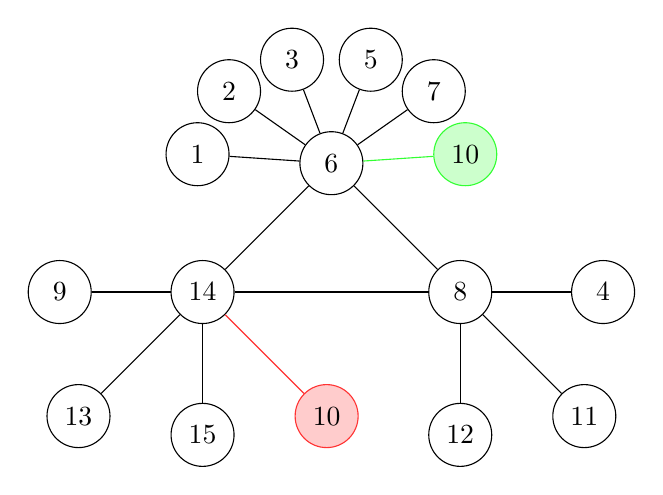
\begin{tikzpicture}[main/.style = {draw, circle,minimum size=0.8cm}]
\node[main] (6) {6};
\node[main] (8) [below right=1.5cm of 6] {8};
\node[main] (14) [below left=1.5cm of 6] {14};

\node[main] (1) [above=of 6,xshift=-1.7cm,yshift=-1.7cm] {1};
\node[main] (2) [above=of 6,xshift=-1.3cm,yshift=-0.9cm] {2};
\node[main] (3) [above=of 6,xshift=-0.5cm,yshift=-0.5cm] {3};
\node[main] (5) [above=of 6,xshift=0.5cm,yshift=-0.5cm] {5};
\node[main] (7) [above=of 6,xshift=1.3cm,yshift=-0.9cm] {7};
\node[main] (10) [above=of 6,xshift=1.7cm,yshift=-1.7cm,draw=green!80,fill=green!20] {10};

\node[main] (4) [right=of 8] {4};
\node[main] (11) [below right=of 8] {11};
\node[main] (12) [below=of 8] {12};

\node[main] (9) [left=of 14] {9};
\node[main] (13) [below left=of 14] {13};
\node[main] (15) [below=of 14] {15};
\node[main] (10-2) [below right=of 14,draw=red!80,fill=red!20] {10};

\draw[-] (8) -- (6);
\draw[-] (14) -- (6);
\draw[-] (8) -- (14);

\draw[-] (1) -- (6);
\draw[-] (2) -- (6);
\draw[-] (3) -- (6);
\draw[-] (5) -- (6);
\draw[-] (7) -- (6);
\draw[-,draw=green!80] (10) -- (6);

\draw[-] (4) -- (8);
\draw[-] (11) -- (8);
\draw[-] (12) -- (8);

\draw[-] (9) -- (14);
\draw[-] (13) -- (14);
\draw[-] (15) -- (14);
\draw[-,draw=red!80] (10-2) -- (14);
\end{tikzpicture}
\caption{A graph of the optimal ILP solution. The 10 coloured red indicates the result of the intuitive algoritm while the 10 coloured green indicates the result of the ILP solution.}
\label{ILPSol}
\end{figure}
\newpage

\section{Expanded algorithm}
The package delivery problem is set out into a data set where only the cost per package and the amount of packages send and received are given. To make this problem more realistic a situation is made where all the packages are collected and distributed using a bus. In this particular case, a bus can hold up to and including a total of one hundred packages~\cite{Packages per bus}. If more packages are needed to move every package, the delivery company will have to send two or more busses. Between the hubs, the company is able to use cargo trucks, such that everything can be send in one vehicle.
This scenario is translated into the algorithm by letting all factors of moving packages to 1 and multiplying this by the amount of busses that are necessary. 


    \subsection{Intuitive algorithm result}
    
        By evaluating the expanded intuitive algorithm a separation is made between the different intuitive algorithms used in Chapter~\ref{Inuitive algorithms}. The expansion of the model will likewise as the standard data have a result which is a combination of the multiple intuitive algorithms. 


        \subsubsection{Algorithm used for the collection costs}
            For the expanded algorithm the same method will be used as in chapter~\ref{Collection of packages}. By adding a city as hub one by one and adding the city as a hub when the costs are lowered, the program is able to make a list of how many times cities are used as hub. With this the cities that are overall valuable to transform into a hub will stand out.
            
             \begin{table}[h!]
                \begin{center}
                \begin{tabular}{|p{3cm}|p{3cm}|p{3cm}|}
                    \hline
                    \multicolumn{3}{|c|}{Amount of times cities are used as hubs} \\
                    \hline
                    City used as hub & Using only collection cost & Using total cost\\
                    \hline
                    1 &  5 & 4 \\
                    \hline
                    2 & 7   & 12 \\
                    \hline
                    3& 6 & 7\\
                    \hline
                    4  & 1 & 1 \\
                    \hline
                    5 & 7 & 7\\
                    \hline
                    6 & 1 & 10   \\
                    \hline
                    7 & 1& 2 \\
                    \hline
                    8 & 1 & 1 \\
                    \hline
                    9 &  10& 10 \\
                    \hline
                    10 & 11 & 12 \\
                    \hline
                    11 & 1& 1 \\
                    \hline
                    12 & 1 & 1 \\
                    \hline
                    13 & 2& 1 \\
                    \hline
                    14 & 14& 14 \\
                    \hline
                \end{tabular}
                \end{center}
                \caption{Table of the amount of times each city is used as a hub in every combination using the large data set for the expanded algorithm}
                \label{amount of times hubs are used in collection expanded algorithm} 
            \end{table}
            
            Applying this data to the original algorithm the following hubs could be preferable.
            
             \begin{table}[h!]
                \begin{center}
                    \begin{tabular}{ |p{3cm}|p{3cm}|p{4cm}|}
                        \hline
                        \multicolumn{3}{|c|}{Cost and combination of hubs with certain input} \\
                        \hline
                        Input into the algorithm & Output -  collection Cost (€ x 10^3) & Output - total Cost (€ x 10^3)\\
                        \hline
                        [14] &  78.3 | [14, 1, 3] & 153.4| [14, 1, 2, 3, 6]  \\
                        \hline
                        [10] & 76.1 | [10, 2, 14]   & 139.5 | [10, 2, 14] \\
                        \hline
                        [9,10 ]& 88.4 | [6, 10, 2, 14] & 148.8 |  [9, 10, 2, 14]\\
                        \hline
                        [6, 14] &  66.6 | [6, 14]  &  131.7 | [6, 14] \\
                        \hline
                        [6, 14, 8] & 75.6 | [2, 10, 14] & 136.3 | [6,14,8]  \\
                        \hline
                    \end{tabular}
                \end{center}
            \caption{Table of the amount of times each city is used as a hub in every combination}
            \label{amount of times hubs are used in collection} 
            \end{table}
            
            This table shows that most likely turning cities 6 and 14 into hubs will result into a low cost. Moreover, cities 2, 10 and 8 also have a high probability of ending up in the final result.

    
        \subsubsection{Algorithm used for transfers between hubs}
            The algorithm that was used in subsection \ref{sssec:num1} on page \pageref{sssec:num1} will be implemented for this situation (more realistic) where the packages are collected and distributed using a bus. We will illustrate this by using the large data assignment. 

            \begin{table}[h!]
            \begin{tabular}{|p{3cm}|p{3cm}|p{3cm}|}
            \hline
            nodes that are hubs & flow of parcels to itself (last node) & Total cost (€ x 10^3) \\
            \hline
            [14] &  181 & 404.3 \\
            \hline
            [14,2]   & 39 & 282.4 \\
            \hline
            [14,2,15] & 26 & 273.1 \\
            \hline
            [14,2,15,6]  & 18 & 228.9 \\
            \hline
            [14,2,15,6,13] & 18 & 222.2\\
            \hline
            [14,2,15,6,13,4] & 11 & 213.6   \\
            \hline
            [14,2,15,6,13,4,3] & 9 & 214.9   \\
            \hline
            [14,2,15,6,13,4,3,9] & 9 & 218.5    \\
            \hline
            [14,2,15,6,13,4,3,9,7] & 9 & 222.9    \\
            \hline
            \end{tabular}
            \caption{Table of nodes that were used as hubs and the associated costs}
            \end{table}

The cheapest situation here is where we have 6 hubs in nodes 2,4,6,13,14,15, the total cost in this situation is €213.621 which is €57086 more expensive than before. An explanation for this is that the packages are not sent on one go, but in two or more times, which would ultimately lead to more costs. There is also a big difference in the locations of the hubs. First there were 4 (2,6,14 and 15) hubs and now two extra hubs are being established. In the following chapters the other algorithms will be implemented and combined so that in the end an optimal situation arises.

\subsubsection{Algorithm used for distribution}
The algorithm used for distribution cost minimisation for the addition to the problem is identical to the one in section \ref{Distribution}. The only modification is to the cost function. Running the algorithm based on distribution costs, given the change, results in table \ref{tab:DistAlgExp}. Again, the first column represents which city got chosen to add to the list of hubs and the costs have been expressed in thousands rounded to one decimal for readability.

\begin{table}[h!]
    \centering
    \begin{tabular}{||c|c|c||}
    \hline
        Chosen hub & Total distribution costs (€ x 10^3) & Total costs (€ x 10^3)  \\
    \hline
    \hline
        14 & 81.2 & 165.4 \\
        \hline
        3 & 45.2 & 136.5 \\
        \hline
        8 & 37.1 & 141.3 \\
        \hline
        2 & 29.5 & 146.3 \\
        \hline
        9 & 22.3 & 154.1 \\
        \hline
        4 & 17.5 & 164.0 \\
        \hline
        7 & 13.8 & 169.3 \\
        \hline
        1 & 11.0 & 179.9 \\
        \hline
        10 & 8.7 & 192.1 \\
        \hline
        13 & 6.9 & 201.1 \\
        \hline
        6 & 5.0 & 211.4 \\
        \hline
        12 & 3.5 & 220.0 \\
        \hline
        5 & 2.0 & 230.1 \\
        \hline
        11 & 0.9 & 243.8 \\
        \hline
        15 & 0 & 253.1 \\
        \hline
    \end{tabular}
    \caption{\centering Order in which the cities got added as hubs by the algorithm based on distribution costs with the expanded problem}
    \label{tab:DistAlgExp}
\end{table}
This result differs quite a bit from the results of section \ref{Distribution}. There are some elements that remain the same, such as the distribution costs decreasing for each added hub and the total costs decreasing at first but increasing later. However, the order in which hubs gets added is quite different. In this case, an optimal solution would be turning cities 3 and 14 into hubs.

Once again, the algorithm is repeated but instead with a focus on the total costs. The results can be seen in table \ref{tab:DistAlgExp2}. Notably, just as in section \ref{Distribution}, we see that cities 2, 6, 8 and 14 are first to be chosen, though 10 is one of the last to be added in this case. The optimal solution in this case also only consists of 2 hubs, namely 6 and 14. 

\begin{table}[h]
    \centering
    \begin{tabular}{||c|c||}
    \hline
        Chosen hub & Total costs (€ x 10^3) \\
    \hline
    \hline
        14 & 165.4 \\
        \hline
        6 & 131.7 \\
        \hline
        2 & 133.2 \\
        \hline
        8 & 137.6 \\
        \hline
        13 & 144.4 \\
        \hline
        12 & 153.2 \\
        \hline
        5 & 162.0 \\
        \hline
        11 & 172.2 \\
        \hline
        4 & 182.5 \\
        \hline
        1 & 193.0 \\
        \hline
        3 & 203.9 \\
        \hline
        7 & 216.6 \\
        \hline
        9 & 223.0 \\
        \hline
        10 & 243.8 \\
        \hline
        15 & 253.1 \\
        \hline
    \end{tabular}
    \caption{\centering Order in which the cities got added as hubs by the algorithm based on total costs with the expanded problem}
    \label{tab:DistAlgExp2}
\end{table}

\subsection{ILP result}
(This part of the expanded algorithm is still being worked on)

\subsection{Difference between the two methods}
(This section is still being worked on)

\newpage
\section{Conclusion}

%we moeten hier de opdracht nog even uitleggen opnieuw // ook in het begin duidelijker verwoorden 
Looking back at the report, the main goal is evaluated. The aim was to create an algorithm which can find a near to perfect or at least a good solution to the package delivery problem. This problem is based on the delivery and collection of packages send between different cities. For each of these cities the option arises to build a so called hub. It is only possible to send packages from and to hubs. Hereby it is important to notice that it is not allowed to send a package between two cities if neither of them is a hub. 

It is preferable to create this algorithm to get a feel for which hubs will give the lowest total cost for the package delivery company. This is due to the fact that there already is an ILP solver which, while it takes quite a long time to run, gives the exact best options for the placement of hubs.  
Out of the combination of the multiple intuitive algorithms it has shown that building hubs in cities 6, 8 and 14 will give one of the lowest possible amount of money. With this combination the total cost results into €144.522 euros. When compared to the exact result, the ILP solver gives the same cities as hubs, namely 6, 8 and 14, but reaches a lower overall cost. The solver changes the connection from city 10 to hub 14 instead of hub 6, which is used in the intuitive algorithms. 

In conclusion, the intuitive algorithm gave a result which was only €163 away form the ILP solver. Given that the intuitive algorithm takes a fraction of the calculating time that the solver uses, it is possible to conclude that the algorithm works extremely well for this specific problem. %stukje over resultaat expanded algorithm
By adding another element into the data set, the problem becomes more realistic. this is done by looking at the way packages are moved around. In this case the restrictions of the problem have been modified such that the packages are moved by busses which can hold up to 100 packages. Even in this expanded algorithm, it shows that the intuitive part assesses the problem quite well. 

\newpage
\section{Bibliography}
\begin{thebibliography}{9}

\bibitem{Packages per bus}
(2016) \textit{Omroepwest}
\url{omroepwest.nl/nieuws/3313393/Tachtig-tot-110-pakketten-per-bus-bezorgers-hebben-het-druk-vlak-voor-Kerstmis}



\end{thebibliography}

\newpage

\appendix
\section{ILP definition}
\label{ILPDef}
\subsection*{Input}
\begin{align*}
c_{ij} &= \text{cost between city i and j}  &i,j \in N\\
w_{ij} &= \text{flow between city i and j} &i,j \in N\\
f_{i} &= \text{cost to turn city i into a hub} &i \in N\\
\chi &= \text{collection cost multiplier} \\
\alpha &= \text{transfer cost multiplier} \\
\delta &= \text{distribution cost multiplier} \\
\end{align*}

\subsection*{Variables}
\begin{align*}
e_{ik} &=
\begin{cases} 
1, & \text{if city i is assigned to hub k} \quad i=1,2,\ldots,N \quad j=1,2,\ldots,N  \\ 
0, & \text{otherwise} 
\end{cases} \\
y_{ijkl} &=
\begin{cases} 
1, & \text{if there is a path } i \rightarrow k \rightarrow l \rightarrow j \quad i=1,2,\ldots,N \quad j=1,2,\ldots,N  \\ 
0, & \text{otherwise} 
\end{cases} \\
\end{align*}

\subsection*{Objective function}
$$min\,z=\sum^N_{i=1}\sum^N_{j=1}\sum^N_{k=1}\sum^N_{l=1}(w_{ij}(\chi c_{ik}+\alpha c_{kl}+\delta c_{lj})y_{ijlk} + \sum^N_{k=1}f_{k}e_{kk}$$

\subsection*{Constraints}
\begin{align*}
\sum^N_{k=1}e_{ik} &= 1 &i \in N \\
e_{ik} & \leq e_{kk} &i,k \in N \\
y_{ijkl} &\leq e_{ik} &i,j,k,l \in N \\
y_{ijkl} &\leq e_{jl} &i,j,k,l \in N \\
y_{ijkl} &\geq e_{ik} + e_{jl} - 1 &i,j,k,l \in N \\
\sum^N_{k=1}f_k e_{kk} &\geq 1
\end{align*}

\newpage

\section{ILP Python implementation}
\label{ILPPyth}
This version of the implementation is specifically for the large data set. The implementation for the small data set is identical apart from some of the input.
\begin{verbatim}
    import pandas as pd
import pulp as p
import numpy as np
#Input
col = 3
trns = 1
dist = 2
cities = range(15)

file = 'Large.xlsx'
xls = pd.ExcelFile(file)

flow = pd.read_excel(xls, 'w')
flow = flow.values[:,1:]

cost = pd.read_excel(xls, 'c')
cost = cost.values[:,1:]

hub_cost = pd.read_excel(xls, 'f')
hub_cost = hub_cost.values[:,1]
hub_cost = np.append([13530], hub_cost)

o = dict()
d = dict()
for i in cities:
    o[i] = p.lpSum(flow[i][j] for j in cities)
    d[i] = p.lpSum(flow[j][i] for j in cities)

#Creating the model
Parcel = p.LpProblem('ParcelDelivery', p.LpMinimize)

#Variables
e = p.LpVariable.dicts('hasEdge', ((i,k) for i in cities
                                         for k in cities), cat='Binary')
#1 if city i is assigned to hub k, 0 otherwise

y = p.LpVariable.dicts('Flow', ((i,j,k,l) for i in cities
                                          for j in cities
                                          for k in cities
                                          for l in cities), cat='Binary')
#1 if i->k->l->j is the path from i to j, 0 otherwise

#Objective function

Parcel += p.lpSum(flow[i][j]*(col*cost[i][k]+
                           trns*cost[k][l]+dist*cost[l][j])*y[(i,j,k,l)]
               for i in cities
               for j in cities
               for k in cities
               for l in cities) + p.lpSum(hub_cost[k]*e[k,k] for k in cities)


#Constraints
for i in cities:
    Parcel += p.lpSum(e[(i,k)] for k in cities) == 1
#Each city i is connected to exactly one hub k.
    
    for k in cities:
        Parcel += e[(i,k)] <= e[(k,k)]
#There can only be connections from i to k if k is connected to itself
#(meaning k is a hub)
        
        for j in cities:
            for l in cities:
                Parcel += y[(i,j,k,l)] <= e[(i,k)]
                Parcel += y[(i,j,k,l)] <= e[(j,l)]https://www.overleaf.com/project/607ecb97092dbc483a588800
                Parcel += y[(i,j,k,l)] >= e[(i,k)] + e[(j,l)] - 1
#With these constraints: y[(i,j,k,l)] = e[(i,k)]*e[(j,l)]

Parcel += p.lpSum(e[k,k] for k in cities) >= 1
#There must be at least one hub
    
solver = p.CPLEX_CMD()
res = Parcel.solve(solver)
print("status:", res)
print("OPT:", p.value(Parcel.objective))
\end{verbatim}

\end{document}
